\documentclass{standalone}
\usepackage{tikz}
\usetikzlibrary{angles,quotes}
\begin{document}
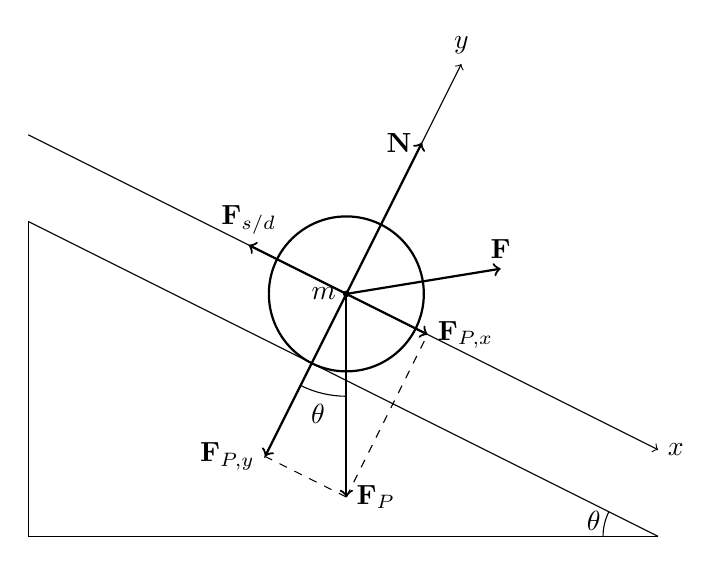
\begin{tikzpicture}[scale=2]
    \draw[-](0,2)coordinate(a)--(4,0)coordinate(b);
    \draw[-](0,2)--(0,0)coordinate(c);
    \draw[-](0,0)--(4,0);

    \coordinate(m)at(2.02,1.54);
    \filldraw[black](m)circle(0.5pt);
    \draw[thick](m)circle(0.492);

    \draw[->](0,2.55)--(4,0.55)node[right]{$x$};
    \draw[->](1.5,0.5)--(2.75,3)node[above]{$y$};

    \draw[->,thick](m)node[left]{$m$}--(2.02,0.25)coordinate(P)node[right]{$\mathbf{F}_P$};
    \draw[dashed](P)--(1.504,0.508)coordinate(Py);
    \draw[->,thick](m)--(Py)node[left]{$\mathbf{F}_{P,y}$};
    \draw[dashed](P)--(2.536,1.282)coordinate(Px);
    \draw[->,thick](m)--(Px)node[right]{$\mathbf{F}_{P,x}$};
    \draw[->,thick](m)--(1.4,1.85)node[above]{$\mathbf{F}_{s/d}$};
    \draw[->,thick](m)--(3,1.7)node[above]{$\mathbf{F}$};
    \draw[->,thick](m)--(2.5,2.5)node[left]{$\mathbf{N}$};


    \pic["$\theta$", draw, angle eccentricity=1.2, angle radius=1.3cm]{angle=Py--m--P};
    \pic["$\theta$", draw,angle eccentricity=1.2, angle radius=0.7cm]{angle=a--b--c};
\end{tikzpicture}
\end{document}